\documentclass[11pt,aspectratio=169, professionalfonts]{beamer}

\usepackage{tasks}
\usepackage{multicol}
\usepackage{amsmath}
\usepackage{amssymb}
\usepackage{vwcol}
\usepackage{python}
\usepackage[backend=biber, style=numeric,sorting=none]{biblatex}


\usepackage{tikz}
\usepackage{tikz-qtree}
%\usepackage{multirow}
\usepackage{wrapfig}
\usepackage{tcolorbox}
\usepackage{rotating}
%\usepackage{lmodern}% http://ctan.org/pkg/lm
\usepackage{anyfontsize}
\usepackage{algorithm,algorithmic}
%\usepackage[ruled,vlined]{algorithm2e}
%\usepackage{mathptmx}
%\usepackage{mathtools}
%\usepackage{pgfplots}
%\usepackage{pgfplotstable}
%\usepackage{outlines}
\usepackage{venndiagram}
% \DeclareGraphicsExtensions{.pdf,.png}
\usepackage{listings}
%\usepackage{hhline}
\usepackage{hyperref}
\usepackage{soul, xcolor}
\usepackage{graphicx}
\usepackage{color, colortbl}
\usepackage{tikz}
\usepackage[absolute,overlay]{textpos}
%\usepackage{algpseudocode}
\usepackage{relsize}
\usepackage{venndiagram}
%\usepackage[framemethod=TikZ]{mdframed}
%\usepackage{xparse}
%\usepackage{mdframed}
% \usepackage{accents}
% \usepackage[T1]{fontenc}
%\usepackage{transparent}
%\usepackage{varwidth}
% \usepackage{mwe} % provides example image

% \usepackage{emoji}
% \setemojifont{Apple Color Emoji}  % Optional
\definecolor{gold}{RGB}{255,215,0}
\definecolor{myblue}{rgb}{0.0,0.125,0.294}
\definecolor{beamer_title_color}{rgb}{1.0, 0.576,0.0}%\usepackage{enumitem}
\normalfont
%\input{/Users/ram/Documents/GitHub/NLProc/Latex/ColorCodes.tex}
% Override palette coloring with secondary
\setbeamercolor{subsection in head/foot}{,fg=white}

\setbeamercolor{normal text}{fg=white,bg=black}

\setbeamercolor{structure}{fg=white}
\setbeamercolor{definition}{fg=white}

%\setbeamercolor{alerted text}{fg=red!85!black}

%\setbeamercolor{item projected}{use=item,fg=black,bg=item.fg!35}

\setbeamercolor{note page}{bg=white}
\setbeamercolor{title}{bg=black, fg=yellow}
\setbeamercolor{author}{bg=black, fg=white}
\setbeamercolor{subtitle}{bg=black, fg=white}
\setbeamercolor{frametitle}{fg=orange,bg=black}
\setbeamertemplate{frametitle}{%
\usebeamerfont{frametitle} \MakeUppercase{\insertframetitle}%
\vphantom{g}% To avoid fluctuations per frame
\hrule% Uncomment to see desired effect, without a full-width hrule
\par% <-- added

{\color{white}\hrulefill}
}

\addtobeamertemplate{navigation symbols}{}{%
	\usebeamerfont{footline}%
	\usebeamercolor[fg=yellow]{footline}%
	\hspace{1em}%
	\insertframenumber/\inserttotalframenumber
}



\setbeamertemplate{footline}
{
	\leavevmode%
	\hbox{%
		\begin{beamercolorbox}[wd=.333333\paperwidth,ht=2.25ex,dp=1ex,center]{subsection in head/foot}%
			\usebeamerfont{subsection in head/foot}\insertsection
		\end{beamercolorbox}%
		\begin{beamercolorbox}[wd=.333333\paperwidth,ht=2.25ex,dp=1ex,center]{subsection in head/foot}%
			\usebeamerfont{title in head/foot}\insertshorttitle
		\end{beamercolorbox}%
		\begin{beamercolorbox}[wd=.333333\paperwidth,ht=2.25ex,dp=1ex,right]{section in head/foot}%
			\usebeamerfont{date in head/foot}\insertshortdate{}\hspace*{2em}
			\insertframenumber{} / \inserttotalframenumber\hspace*{2ex}
	\end{beamercolorbox}}%
	\vskip0pt%
}
\makeatother

\usetikzlibrary{chains,shapes}
\tikzstyle{MyText} = [text width=0.5cm,text centered]
\usetikzlibrary{decorations.text}
\setlength{\columnseprule}{0.2pt}
\def\columnseprulecolor{\color{yellow}}
\usepackage{nicefrac}
\usetikzlibrary{automata, shapes.geometric,circuits,positioning,shapes,arrows,fit,calc,decorations.pathmorphing,decorations}
% or whatever (possibly just delete it)

\usepackage[printwatermark=true]{xwatermark}



%\SetWatermarkText{\includegraphics{JCRLogo.png}}
%\setbeamertemplate{background}{
%	\tikz[overlay,remember picture]\node[opacity=0.04]at (current page.center){\includegraphics[width=4cm]{JCRLogo}};
%	}
\lstset{
backgroundcolor=\color{myblue},   % choose the background color; you must add \usepackage{color} or \usepackage{xcolor}; should come as last argument
basicstyle=\ttfamily\scriptsize,        % the size of the fonts that are used for the code
breakatwhitespace=false,         % sets if automatic breaks should only happen at whitespace
breaklines=false,                 % sets automatic line breaking
captionpos=b,                    % sets the caption-position to bottom
commentstyle=\color{green!25},    % comment style
deletekeywords={...},            % if you want to delete keywords from the given language
escapeinside={\%*}{*)},          % if you want to add LaTeX within your code
extendedchars=true,              % lets you use non-ASCII characters; for 8-bits encodings only, does not work with UTF-8
%frame=single,	                   % adds a frame around the code
keepspaces=true,                 % keeps spaces in text, useful for keeping indentation of code (possibly needs columns=flexible)
keywordstyle=\color{orange},       % keyword style
basicstyle=\small\ttfamily
morekeywords={*,...},            % if you want to add more keywords to the set
numbers=left,                    % where to put the line-numbers; possible values are (none, left, right)
numbersep=5pt,                   % how far the line-numbers are from the code
numberstyle=\tiny\color{cyan}, % the style that is used for the line-numbers
rulecolor=\color{white},         % if not set, the frame-color may be changed on line-breaks within not-black text (e.g. comments (green here))
showspaces=false,                % show spaces everywhere adding particular underscores; it overrides 'showstringspaces'
showstringspaces=false,          % underline spaces within strings only
showtabs=false,                  % show tabs within strings adding particular underscores
stepnumber=0,                    % the step between two line-numbers. If it's 1, each line will be numbered
stringstyle=\color{green},     % string literal style
tabsize=4,	                   % sets default tabsize to 2 spaces
%title=\lstname                   % show the filename of files included with \lstinputlisting; also try caption instead of title
belowskip=-5pt,
basicstyle=\ttfamily,
keywordstyle = \color{yellow},
language=Python,
}



\graphicspath{{Images/}}



\hypersetup{
colorlinks=true,
linkcolor=blue,
filecolor=magenta,
urlcolor=cyan,
}

\urlstyle{same}

\newsavebox\mybox

\newwatermark*[
angle=0,
allpages=true,
scale=0.1,
xpos=-5.75,
ypos=0
]{\usebox\mybox}


\tikzstyle{mybox} = [draw=white, fill=blue!75, very thick,
rectangle, rounded corners, inner sep=10pt, inner ysep=10pt]
\tikzstyle{fancytitle} =[draw=white,fill=blue!75, text=white, ellipse, very thick]



\newcommand{\ffbox}[1]{%
	{% open a group for a local setting
		\setlength{\fboxsep}{-2\fboxrule}% the rule will be inside the box boundary
		\fbox{\hspace{1.2pt}\strut#1\hspace{1.2pt}}% print the box, with some padding at the left and right
	}% close the group
}

\tikzset{
	NNnode/.pic={
		\pgfmathsetmacro\RecH{2}
		\pgfmathsetmacro\RecW{\RecH/10}
		\coordinate (-ll) at (-\RecW/2,-\RecH/2);
		\coordinate (-ur) at (\RecW/2,\RecH/2);
		\coordinate (-lr) at (-ll-|-ur);
		\coordinate (-ul) at (-ll|--ur);
		\path (-ul) -- (-ur) coordinate[midway] (-north);
		\path (-ll) -- (-lr) coordinate[midway] (-south);
		\path (-ll) -- (-ul) coordinate[midway] (-west);
		\path (-ur) -- (-lr) coordinate[midway] (-east);

		\begin{scope}[shift={(-\RecW/2,-\RecH/2)}]
			\draw (-ll) rectangle (-ur);
			\foreach \y in {0.05,0.5,0.75,0.85,0.95}
			\draw (0.5*\RecW,\RecH*\y) circle[radius=0.3*\RecW];
			\foreach \y in {0.275,0.625} {
				\fill (\RecW*0.4,\y*\RecH-0.1*\RecW) rectangle (0.6*\RecW,\y*\RecH-0.3*\RecW);
				\fill (\RecW*0.4,\y*\RecH+0.1*\RecW) rectangle (0.6*\RecW,\y*\RecH+0.3*\RecW);
			}
		\end{scope}
	}
}
\newenvironment{WrapText}[1][c]
{\wrapfigure{}{0.35\textwidth}\tcolorbox}
{\endtcolorbox\endwrapfigure}


\tikzstyle{decision} = [diamond, draw, text width=4.5em, text badly centered, node distance=3.5cm, inner sep=0pt]
\tikzstyle{block} = [rectangle, draw, text width=4em, text centered, rounded corners, minimum height=4em, node distance=0.5cm,minimum height=5em]
\tikzstyle{hidden} = [rectangle, draw, text width=0.5em, text centered, rounded corners, minimum height=2.5em, node distance=0.6cm,minimum height=2.5em,fill,red,opacity=0.85]
\tikzstyle{cloud} = [draw, ellipse, node distance=3.5cm, minimum height=2em]
\tikzstyle{line} = [draw, -latex']

\tikzstyle{vecArrow} = [thick, decoration={markings,mark=at position
	1 with {\arrow[semithick]{open triangle 60}}},
double distance=1.4pt, shorten >= 5.5pt,
preaction = {decorate},
postaction = {draw,line width=1.4pt, white,shorten >= 4.5pt}]
\tikzstyle{innerWhite} = [semithick, white,line width=1.4pt, shorten >= 4.5pt]

\DeclareMathOperator*{\argmin}{\arg\min}
\DeclareMathOperator*{\argmax}{\arg\max}

\tikzstyle{MyText} = [text width=0.5cm,text centered]


\newcommand\irregularline[2]{%
	let \n1 = {rand*(#1)} in
	+(0,\n1)
	\foreach \a in {0.1,0.2,...,#2}{
		let \n1 = {rand*(#1)} in
		-- +(\a,\n1)
	}
}

\usefonttheme{professionalfonts}
\setbeamercolor{frametitle}{fg=orange}
\setbeamerfont{frametitle}{size=\large}
\beamertemplatenavigationsymbolsempty


\newcommand*\circled[1]{\tikz[baseline=(char.base)]{
		\node[shape=circle,draw,inner sep=1pt] (char) {#1};}}

\setbeamertemplate{section in toc}{%
	\usebeamercolor[fg]{enumerate item}%
	\makebox[2em][l]{\circled{\inserttocsectionnumber}}%
	\parbox[t]{\dimexpr\linewidth-2em}{\inserttocsection}%
}
\setbeamercolor{item projected}{bg=orange}
\setbeamercolor*{item}{fg=orange}


\usepackage{xcolor}
\definecolor{c1}{rgb}{1,1,0} % blue
\definecolor{c2}{rgb}{1,1,1} % light blue
\definecolor{c3}{rgb}{1,1,0} % red blue
\hypersetup{
	linkcolor= {c1}, % internal links
	citecolor={c2}, % citations
	urlcolor={c3} % external links/urls
}

\setbeamercolor{background canvas}{bg=myblue}

%\setbeamercolor{note page}{bg=white}
\setbeamercolor{title}{bg=myblue, fg=gold}
\setbeamercolor{author}{bg=myblue, fg=white}
\setbeamercolor{subtitle}{bg=myblue, fg=white}
\setbeamercolor{frametitle}{fg=beamer_title_color,bg=myblue}
\addbibresource{/Users/ram/Documents/GitHub/NLProc/Latex/Bib/NLP.bib}

\logo{
	\begin{tikzpicture}[remember picture,overlay]
        \node[below left,inner sep=0pt] at (current page.north east) {
           \ifnum\thepage>1 
\includegraphics[width=1.00cm]{Images/TALogo}\fi
        };
      \end{tikzpicture}
      }

\newcommand{\clrtxt}[2]{\textcolor{#1}{#2}}
\newcommand{\keywordclr}[2][yellow]{\textcolor{#1}{#2}}
\newcommand{\headclr}[1]{\textcolor{cyan}{\textbf{\large #1}}\par}

\usepackage{fontspec}
\usepackage[defaultsans,scaled=.95]{opensans}
\renewcommand\seriesdefault{l}
\renewcommand\mddefault{l}
\renewcommand\bfdefault{sb}% or \renewcommand\bfdefault{m}

\title{Text Analytics}
\author{Ramaseshan Ramachandran}
\begin{document}

\frame{\titlepage}

\section{Introduction to Text Analytics}
\begin{frame}{What is Text Analytics?}
\begin{itemize}
    \item Converts unstructured text into insights
    \item Extracts patterns and trends
    \item Uses NLP, machine learning, and statistics
    \item Analyzes data from diverse sources
\end{itemize}
\end{frame}

\begin{frame}{Importance of Text Analytics}
\begin{itemize}
    \item Unstructured text data is vast
    \item Text data is messy and variable
    \item Makes data measurable and valuable
\end{itemize}
\end{frame}

\begin{frame}{Benefits of Text Analytics}
\begin{itemize}
    \item Understand customers and societal trends
    \item Enhance decision-making and planning
    \item Drive engagement and innovation
\end{itemize}
\end{frame}

\section{Key Activities in Text Analytics}
\begin{frame}{Information Retrieval (IR)}

\begin{multicols}{2}
\begin{itemize}
    \item Searches documents and metadata
    \item Extracts relevant data to queries
    \item Applies to large text collections
\end{itemize}
\vfill\null \columnbreak
\begin{itemize}
    \item Boolean Retrieval Model
    \item Vector Space Model (TF-IDF)
    \item Probabilistic Retrieval Model
    \item Latent Semantic Indexing (LSI)
    \item BM25 Algorithm
\end{itemize}

\end{multicols}
\end{frame}

\begin{frame}{Text Classification}
\begin{multicols}{2}
\begin{itemize}
    \item Categorizes text into predefined labels
    \item Applications: spam detection, sentiment analysis
    \item Automates document organization
\end{itemize}
\vfill\null\columnbreak
\begin{itemize}
    \item Naive Bayes Classifier
    \item Support Vector Machines (SVM)
    \item Logistic Regression
    \item Decision Trees and Random Forests
    \item Deep Learning (CNNs, RNNs, Transformers)
\end{itemize}
\end{multicols}
\end{frame}

\begin{frame}{Clustering}
\begin{multicols}{2}
\begin{itemize}
    \item Groups similar texts together
    \item No predefined labels required
    \item Useful for exploratory analysis
\end{itemize}

\vfill\null\columnbreak
\begin{itemize}
    \item K-Means Clustering
    \item Hierarchical Clustering
    \item DBSCAN (Density-Based Clustering)
    \item Gaussian Mixture Models (GMMs)
    \item Spectral Clustering
\end{itemize}
\end{multicols}
\end{frame}

\begin{frame}{Sentiment Analysis}
\begin{multicols}{2}
\begin{itemize}
    \item Determines text’s emotional tone
    \item Classifies as positive, negative, or neutral
    \item Applications: marketing, feedback analysis
\end{itemize}
\vfill\null\columnbreak
\begin{itemize}
    \item Lexicon-Based Approaches
    \item Rule-Based Sentiment Analysis
    \item Machine Learning-Based Approaches
    \item Neural Networks (LSTMs, GRUs, BERT)
    \item Pretrained Models (RoBERTa, GPT)
\end{itemize}
\end{multicols}
\end{frame}

\begin{frame}{Entity Recognition}
\begin{multicols}{2}
\begin{itemize}
    \item Identifies entities in text (e.g., names)
    \item Categorizes into people, places, etc.
    \item Useful for automated content analysis
\end{itemize}
\vfill\null\columnbreak
\begin{itemize}
    \item Hidden Markov Models (HMMs)
    \item Conditional Random Fields (CRFs)
    \item Maximum Entropy Models
    \item Neural Networks (BiLSTM + CRF)
    \item Pretrained Models (SpaCy, Hugging Face)
\end{itemize}
\end{multicols}
\end{frame}

\begin{frame}{Topic Modeling}
\begin{multicols}{2}
\begin{itemize}
    \item Discovers themes in document collections
    \item Applications: summarization, recommendations
\end{itemize}
\vfill \null
\columnbreak
\begin{itemize}
\item[] {\larger \underline{\textit{\color{yellow}Algorithms}}}
    \item Latent Dirichlet Allocation (LDA)
    \item Non-Negative Matrix Factorization (NMF)
    \item Latent Semantic Analysis (LSA)
    \item Gibbs Sampling for LDA
    \item Neural Topic Models (ProdLDA, BERTopic)
\end{itemize}
\end{multicols}
\end{frame}
\section{Advanced Techniques}
\begin{frame}{Other Advanced Techniques}
\begin{itemize}
    \item Word Embedding Models (Word2Vec, GloVe, FastText)
    \item Sentence Embeddings (Sentence-BERT)
    \item Attention Mechanisms
    \item Transformers (BERT, GPT, T5)
    \item Text Summarization (Extractive and Abstractive)
\end{itemize}
\end{frame}

\section{Conclusion}
\begin{frame}{Conclusion}
\begin{itemize}
    \item Text analytics unlocks data potential
    \item Drives decisions and innovation
    \item Benefits industries like finance and healthcare
    \item A variety of algorithms drive text analytics
    \item Techniques range from statistical to neural
    \item Tailor solutions based on use case
\end{itemize}
\end{frame}
\begin{frame}{Word embedding cannot fight with others. Why}
\begin{center}
	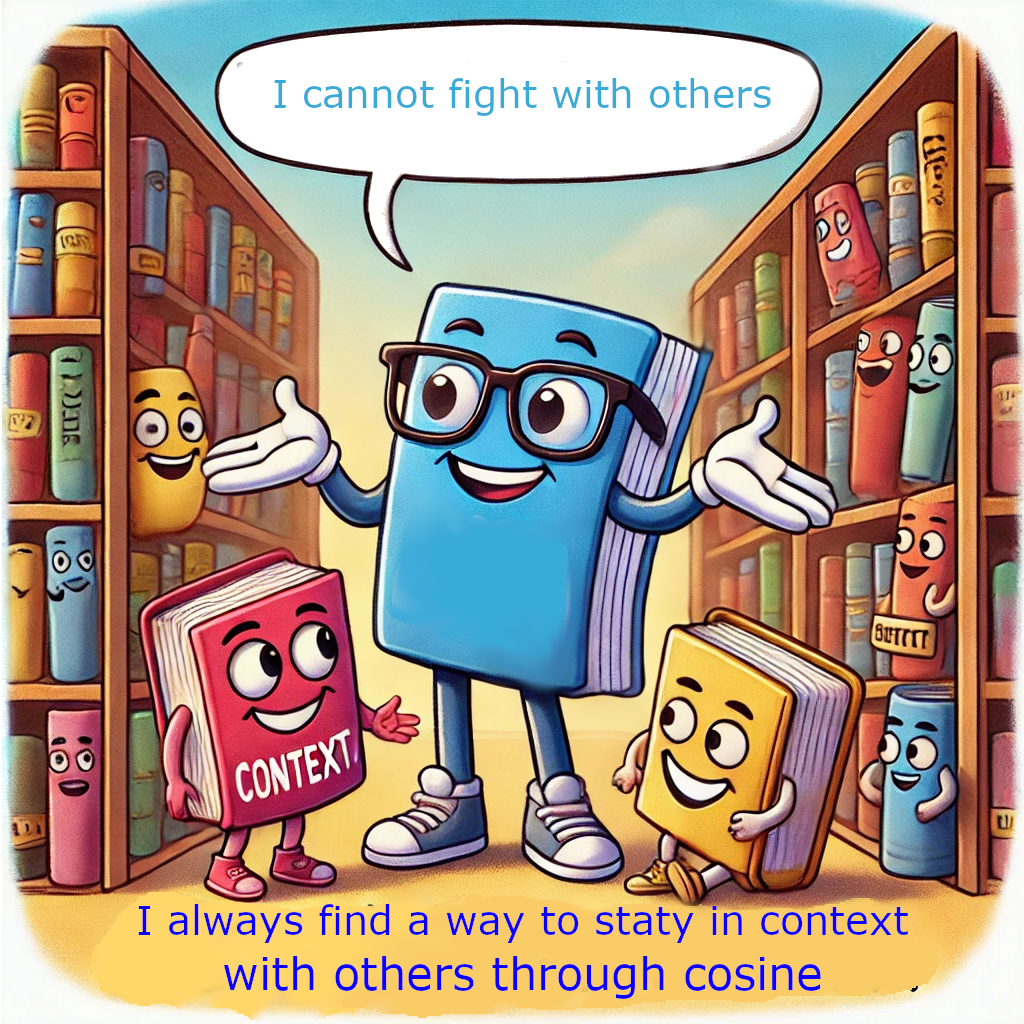
\includegraphics[width=0.55\linewidth]{Images/TAJoke1}
\end{center}

\end{frame}


	% Slide 2: What is Scikit-Learn?
	\begin{frame}{What is Scikit-Learn?}
		\begin{itemize}
			\item {\color{yellow}Definition:} Scikit-learn is a Python library for machine learning, providing tools for:
			\begin{itemize}
				\item Classification
				\item Regression
				\item Clustering
				\item Dimensionality reduction
				\item Preprocessing and more
			\end{itemize}
			\item \textbf{Key Features:}
			\begin{itemize}
				\item Built on NumPy, SciPy, and matplotlib
				\item Simple and efficient tools for predictive data analysis
				\item Open source
			\end{itemize}
		\end{itemize}
	\end{frame}
	
	% Slide 3: Why Use Scikit-Learn in Text Analytics?
	\begin{frame}{Why Use Scikit-Learn in Text Analytics?}
		\begin{itemize}
			\item \textbf{Text Analytics Focus:}
			\begin{itemize}
				\item Natural Language Processing (NLP) tasks
				\item Feature extraction (e.g., bag-of-words, TF-IDF)
				\item Building predictive models
			\end{itemize}
			\item \textbf{Advantages:}
			\begin{itemize}
				\item Wide range of algorithms (SVMs, Naive Bayes, etc.)
				\item User-friendly API for rapid prototyping
				\item Extensive documentation and community support
			\end{itemize}
		\end{itemize}
	\end{frame}
	
	% Slide 4: Common Use Cases in Text Analytics
	\begin{frame}{Common Use Cases in Text Analytics}
		\begin{itemize}
			\item \textbf{Examples:}
			\begin{itemize}
				\item Spam detection
				\item Sentiment analysis
				\item Topic modeling
				\item Document classification
			\end{itemize}
			\item \textbf{Techniques:}
			\begin{itemize}
				\item Preprocessing: Tokenization, stemming, lemmatization
				\item Vectorization: TF-IDF or CountVectorizer
				\item Model training: Logistic regression, SVMs, etc.
			\end{itemize}
		\end{itemize}
	\end{frame}
	
	% Slide 5: Typical Workflow in Scikit-Learn
	\begin{frame}{Typical Workflow in Scikit-Learn}
		\begin{enumerate}
			\item \textbf{Data Preprocessing:}
			\begin{itemize}
				\item Cleaning text data (e.g., removing stop words)
				\item Vectorization (e.g., TF-IDF)
			\end{itemize}
			\item \textbf{Model Selection:}
			\begin{itemize}
				\item Choosing an algorithm (e.g., Naive Bayes)
			\end{itemize}
			\item \textbf{Model Training:}
			\begin{itemize}
				\item \texttt{model.fit(X\_train, y\_train)}
			\end{itemize}
			\item \textbf{Model Evaluation:}
			\begin{itemize}
				\item Metrics like accuracy, precision, recall
			\end{itemize}
			\item \textbf{Prediction:}
			\begin{itemize}
				\item \texttt{model.predict(X\_test)}
			\end{itemize}
		\end{enumerate}
	\end{frame}
	
	% Slide 6: Example: Text Classification Workflow
	\begin{frame}{Example: Text Classification Workflow}
		\textbf{Dataset:} Sentiment Analysis on Product Reviews
		\begin{enumerate}
			\item Load dataset
			\item Preprocess text (lowercase, remove punctuation, etc.)
			\item Vectorize with TF-IDF
			\item Train model (e.g., Logistic Regression)
			\item Evaluate using accuracy and F1-score
		\end{enumerate}
\end{frame}
		\begin{frame}[fragile]{Code Example:}
		\begin{lstlisting}
from sklearn.feature_extraction.text import TfidfVectorizer
from sklearn.model_selection import train_test_split
from sklearn.linear_model import LogisticRegression
from sklearn.metrics import accuracy_score

vectorizer = TfidfVectorizer()
X = vectorizer.fit_transform(text_data)
X_train, X_test, y_train, y_test = train_test_split(X, labels, test_size=0.2)
model = LogisticRegression()
model.fit(X_train, y_train)
predictions = model.predict(X_test)
print("Accuracy:", accuracy_score(y_test, predictions))
		\end{lstlisting}
	\end{frame}
	
	% Slide 7: Strengths and Limitations
	\begin{frame}{Strengths and Limitations}
		\begin{itemize}
			\item \textbf{Strengths:}
			\begin{itemize}
				\item Easy to use and integrate
				\item Extensive support for text-related tasks
				\item Scalability for moderate-sized datasets
			\end{itemize}
			\item \textbf{Limitations:}
			\begin{itemize}
				\item Not designed for deep learning
				\item Limited support for out-of-core learning
			\end{itemize}
		\end{itemize}
	\end{frame}
	
	% Slide 8: Resources to Learn More
	\begin{frame}{Resources to Learn More}
		\begin{itemize}
			\item Official Documentation: \url{https://scikit-learn.org}
			\item Tutorials:
			\begin{itemize}
				\item "Getting Started with Scikit-Learn" (Blog/Video)
				\item Kaggle courses on ML
			\end{itemize}
			\item Recommended Books:
			\begin{itemize}
				\item \textit{Python Machine Learning} by Sebastian Raschka
				\item \textit{Introduction to Machine Learning with Python} by Andreas Müller
			\end{itemize}
		\end{itemize}
	\end{frame}
	
	% Slide 9: Q&A
	\begin{frame}{Questions \& Answers}
		\centering
		\Large Questions?
	\end{frame}
	


\end{document}